\documentclass[border=1pt]{standalone}
\usepackage{newtxtext,newtxmath}
\usepackage{pgfplots}
\usetikzlibrary{calc}
\pgfplotsset{compat=1.18}
\definecolor{obs}{HTML}{D55E00}
\definecolor{sens}{HTML}{0072B2}
\begin{document}
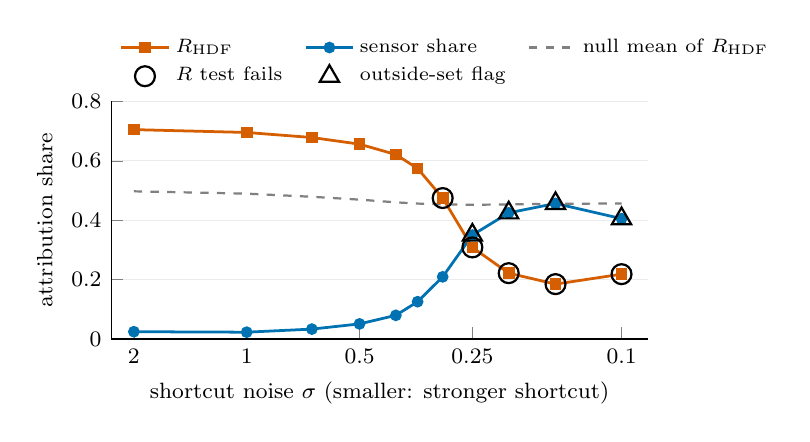
\begin{tikzpicture}
\begin{semilogxaxis}[width=8.4cm, height=4.6cm, x dir=reverse, xmin=0.085, xmax=2.3, ymin=0, ymax=0.8,
  axis x line*=bottom, axis y line*=left, tick label style={font=\footnotesize},
  xtick={2,1,0.5,0.25,0.1}, xticklabels={2,1,0.5,0.25,0.1},
  xlabel={shortcut noise $\sigma$ (smaller: stronger shortcut)}, ylabel={attribution share},
  label style={font=\footnotesize}, ymajorgrids, grid style={black!8},
  legend style={draw=none, fill=none, font=\scriptsize, at={(0.0,1.02)}, anchor=south west, legend columns=3,
                /tikz/every even column/.append style={column sep=6pt}}, legend cell align=left]
\addplot[obs, line width=1pt, mark=square*, mark size=1.6pt] coordinates {(2.0,0.7050) (1.0,0.6954) (0.67,0.6784) (0.5,0.6561) (0.4,0.6211) (0.35,0.5742) (0.3,0.4746) (0.25,0.3084) (0.2,0.2218) (0.15,0.1849) (0.1,0.2184)};
\addlegendentry{$R_{\mathrm{HDF}}$}
\addplot[sens, line width=1pt, mark=*, mark size=1.6pt] coordinates {(2.0,0.0247) (1.0,0.0231) (0.67,0.0335) (0.5,0.0510) (0.4,0.0798) (0.35,0.1258) (0.3,0.2094) (0.25,0.3500) (0.2,0.4248) (0.15,0.4564) (0.1,0.4053)};
\addlegendentry{sensor share}
\addplot[black!50, dashed, line width=0.8pt] coordinates {(2.0,0.4973) (1.0,0.4895) (0.67,0.4789) (0.5,0.4693) (0.4,0.4602) (0.35,0.4560) (0.3,0.4535) (0.25,0.4519) (0.2,0.4533) (0.15,0.4553) (0.1,0.4563)};
\addlegendentry{null mean of $R_{\mathrm{HDF}}$}
\addplot[only marks, mark=o, mark size=3.6pt, black, line width=0.8pt] coordinates {(0.3,0.4746) (0.25,0.3084) (0.2,0.2218) (0.15,0.1849) (0.1,0.2184)};
\addlegendentry{$R$ test fails}
\addplot[only marks, mark=triangle, mark size=4pt, black, line width=0.8pt] coordinates {(0.25,0.3500) (0.2,0.4248) (0.15,0.4564) (0.1,0.4053)};
\addlegendentry{outside-set flag}
\end{semilogxaxis}
\end{tikzpicture}
\end{document}
